% 
% PARTIO SOFTWARE
% Copyright 2010 Disney Enterprises, Inc. All rights reserved
% 
% Redistribution and use in source and binary forms, with or without
% modification, are permitted provided that the following conditions are
% met:
% 
% * Redistributions of source code must retain the above copyright
% notice, this list of conditions and the following disclaimer.
% 
% * Redistributions in binary form must reproduce the above copyright
% notice, this list of conditions and the following disclaimer in
% the documentation and/or other materials provided with the
% distribution.
% 
% * The names "Disney", "Walt Disney Pictures", "Walt Disney Animation
% Studios" or the names of its contributors may NOT be used to
% endorse or promote products derived from this software without
% specific prior written permission from Walt Disney Pictures.
% 
% Disclaimer: THIS SOFTWARE IS PROVIDED BY WALT DISNEY PICTURES AND
% CONTRIBUTORS "AS IS" AND ANY EXPRESS OR IMPLIED WARRANTIES, INCLUDING,
% BUT NOT LIMITED TO, THE IMPLIED WARRANTIES OF MERCHANTABILITY, FITNESS
% FOR A PARTICULAR PURPOSE, NONINFRINGEMENT AND TITLE ARE DISCLAIMED.
% IN NO EVENT SHALL WALT DISNEY PICTURES, THE COPYRIGHT HOLDER OR
% CONTRIBUTORS BE LIABLE FOR ANY DIRECT, INDIRECT, INCIDENTAL, SPECIAL,
% EXEMPLARY, OR CONSEQUENTIAL DAMAGES (INCLUDING, BUT NOT LIMITED TO,
% PROCUREMENT OF SUBSTITUTE GOODS OR SERVICES; LOSS OF USE, DATA, OR
% PROFITS; OR BUSINESS INTERRUPTION) HOWEVER CAUSED AND BASED ON ANY
% THEORY OF LIABILITY, WHETHER IN CONTRACT, STRICT LIABILITY, OR TORT
% (INCLUDING NEGLIGENCE OR OTHERWISE) ARISING IN ANY WAY OUT OF THE USE
% OF THIS SOFTWARE, EVEN IF ADVISED OF THE POSSIBILITY OF SUCH DAMAGES.


\documentclass{article}
\usepackage{graphicx}
\usepackage{fullpage}
\begin{document}
\title{Partio: Tutorial and Documentation}
\author{Andrew Selle}
\maketitle

\section{Introduction}

Partio is a library for manipulating and handling particles. It is designed to be as easy to use as possible while still allowing relatively good performance.  The data model is designed to
accomidate most particle formats in some way.

\section{Data Model}

Partio does not specify how data should be organized in a memory or on the file. It does have a model interface that all particle formats need to implement. This consists of three different
levels of data access

\begin{enumerate}
\item ParticlesHeaders - Number of particles, attribute types and names
\item ParticlesData - Read access to all data
\item ParticlesDataMutable - Write access to all data
\end{enumerate}

Fundamentally a particle is an indexable item that has associated attributes. There can be zero or more attributes, and technically, position is not requires. On the other hand, many of the
file formats (BGEO, GEO, PTC) require position to be present to write a useful file.

\subsection{Attribute Data Types}

There are three data types supported. 
\begin{enumerate}
\item FLOAT - Floating point data, 4 bytes per float
\item VECTOR - Floating point data
\item INT - Integer data type
\end{enumerate}
In addition each attribute is actually an array that can consist of one or more elements. A vector is a special case of a FLOAT and must have a count of 3.  This is to match a common case
where a position is a 3 float value.  (This is modeled loosely after PDB/PDA formats). 

\subsection{Attributes}

Each particle set has a list of attributes that are available. Each of these attributes has a data type and a string representing the name of the attribute.  Particle attributes are
represented by the class \verb|ParticleAttribute|.  A particle class can be queried for individual particle attributes which then become handles that allow stringless (efficient) access to
particle attributes.

\section{Python API}

The python API is designed for ease of use. For speed critical applications, C++ API should be used.  Looping in python is extremely slow.  It is hoped that in the future a mapping to numpy
might be provided to allow manipulating particles in a SIMD fashion.  Nevertheless, python API remains useful for manipulating particles

To use Partio's python API first import partio as
\begin{verbatim}
>>> import partio
\end{verbatim}
Help on functions that are available are shown in 
\begin{verbatim}
>>> help(partio)
\end{verbatim}

\subsection{Creating a Particle Set}

To create a particle set and add a couple of attributes one could write
\begin{verbatim}
particleSet=partio.create()
P=particleSet.addAttribute("position",partio.VECTOR,3)
V=particleSet.addAttribute("velocity",partio.VECTOR,3)
id=particleSet.addAttribute("id",partio.INT,1)
\end{verbatim}
Once this is done, we could add a series of particles that form a circle
\begin{verbatim}
n=30
radiansPer=2*math.pi/n
particleSet.addParticles(n)
for i in range(n):
    particleSet.set(P,i,(math.cos(i*radiansPer),0,math.sin(i*radiansPer)))
    particleSet.set(V,i,(0,0,0))
    particleSet.set(id,i,(i,))
\end{verbatim}
Finally, we can write the particle file into a BGEO by writing 
\begin{verbatim}
partio.write("circle.bgeo",particleSet) # write uncompressed
partio.write("circle.bgeo",particleSet,True) # write compressed
partio.write("circle.bgeo.gz",particleSet) # write compressed
\end{verbatim}
We can then visualize the particle set with
\begin{verbatim}
partview circle.bgeo
\end{verbatim}
giving\\
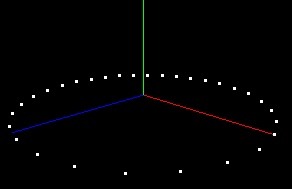
\includegraphics{figures/circleFigure.png}


\subsection{Loading a particle set}

Loading a particle set is relatively easy.  If you only want to know how many particles are available or what headers are available you can do
\begin{verbatim}
>>> pHeaders=partio.readHeaders("circle.bgeo")
\end{verbatim}
If you want everything associated with the file
\begin{verbatim}
>>> p=partio.read("circle.bgeo")
\end{verbatim}
\end{document}

\subsection{Finding nearest neighbors}

A KD-Tree mode is supported in partio.  To use it, you must first sort the particles into a KD-Tree. This is done with the \verb|sort()| function.  Once that is done a query can be done. The
basic query requires a maximum distance to look for particles as well as a maximum number of particles to return. For example, we could read our circle back in and look for particles nearby
(1,0,0) like so:
\begin{verbatim}
p=partio.read("circle.bgeo")
p.sort()
p.findNPoints((1.,0.,0.),.1,3)
\end{verbatim}